\documentclass[12pt,a4paper,french]{article}

\usepackage[utf8]{inputenc}
\usepackage[T1]{fontenc}
\usepackage{lmodern}
%\usepackage{kpfonts}

\usepackage{amsmath,amsfonts,amssymb,amsthm}
\usepackage{tikz}
\usetikzlibrary{calc,intersections,through,backgrounds}
\usepackage{tikz-cd}
\usepackage{tkz-euclide}
\usetkzobj{all}
\usepackage{wrapfig}
\usepackage{enumitem}
\usepackage{stmaryrd}
\usepackage{mdframed}
\usepackage[bookmarks=false,colorlinks,linkcolor=blue,pdfusetitle]{hyperref}
%\usepackage[a4paper,vmargin=1.0cm,hmargin=2cm,includefoot]{geometry}
%\usepackage{lastpage}
%\usepackage{fancyhdr}
%\usepackage{multicol}
%\usepackage[np,autolanguage]{numprint}
\usepackage{babel}

\frenchbsetup{og=«,fg=»}
\pdfminorversion 7
\pdfobjcompresslevel 3
%\count1=\year \count2=\year
%\ifnum\month<8\advance\count1by-1\else\advance\count2by1\fi
%\pagestyle{fancy}
%\cfoot{\textsl{\footnotesize{Année \number\count1/\number\count2}}}
%%\lfoot{\textsl{\footnotesize{LAL 1.3 Vincent-Xavier \textsc{Jumel}}}}
%\rfoot{\textsl{\footnotesize{Page \thepage/ \pageref{LastPage}}}}
%\lhead{}
%\rhead{}
%\renewcommand{\headrulewidth}{0pt}
%\renewcommand{\footrulewidth}{0pt}


\theoremstyle{definition}
\newtheorem{definition}{Définition}
\theoremstyle{plain}
\newtheorem{theoreme}[definition]{Théorème}
\newtheorem{theoremedefinition}[definition]{Théorème et définition}
\newtheorem{proposition}[definition]{Proposition}
\newtheorem{corollaire}[definition]{Corollaire}
\newtheorem{lemme}[definition]{Lemme}
\newtheorem*{exemple}{Exemple}
\newtheorem*{exemples}{Exemples}
\newtheorem*{notation}{Notation}
\theoremstyle{remark}
\newtheorem*{rappel}{Rappel}
\newtheorem*{remarque}{Remarque}
\newtheorem*{remarques}{Remarques}

\setlist[enumerate,1]{label=(\roman*)}
\setlist[itemize,1]{label=\textbullet}

\renewcommand{\k}{\mathbf{k}}
\newcommand{\R}{\mathbf{R}}
\newcommand{\N}{\mathbf{N}}
\newcommand{\K}{\mathbf{K}}
\newcommand{\Q}{\mathbf{Q}}
\newcommand{\Z}{\mathbf{Z}}
\newcommand{\U}{\mathbf{U}}
\newcommand{\C}{\mathbf{C}}
\newcommand{\F}{\mathbf{F}}
\newcommand{\doubleaccent}{\H}
\renewcommand{\H}{\mathbf{H}}
\newcommand{\Fe}{\mathcal{F}}
\newcommand{\E}{\mathbf{E}}
\newcommand{\slcr}{\P}
\renewcommand{\P}{\mathbf{P}}
\newcommand{\Co}{\mathcal{C}}
\renewcommand{\L}{\mathcal{L}}
\newcommand{\Normal}{\mathcal{N}}
\newcommand{\B}{\mathcal{B}}
\newcommand{\parm}{\S}
\renewcommand{\S}{\mathcal{S}}
\newcommand{\M}{\mathcal{M}}
\newcommand{\T}{\mathcal{T}}
\newcommand{\textempty}{\O}
\renewcommand{\O}{\mathcal{O}}
\newcommand{\Sp}{\mathop{Sp}}
\newcommand{\im}{\mathop{Im}}
\newcommand{\Id}{\mathop{Id}\nolimits}
\newcommand{\Card}{\mathop{Card}}
\newcommand{\Aut}{\mathop{Aut}}
\newcommand{\Var}{\mathop{Var}}
\newcommand{\GL}{\mathop{GL}\nolimits}
\newcommand{\SO}{\mathop{SO}\nolimits}
\newcommand{\diff}{\mathop{}\!\mathrm{d}}
\newcommand{\Vect}{\mathop{Vect}\nolimits}
\newcommand{\car}{\mathbf{1}}

\parindent0pt

\usepackage{babel}
\usepackage{draftwatermark}

\everymath{\displaystyle}


\makeatletter
\hypersetup{
  pdftitle={\scantokens\expandafter{\jobname\noexpand}},
  %pdfsubject={Modèle de document LaTeX},
  %pdfkeywords={LaTeX, modèle},
  pdfauthor={Vincent-Xavier Jumel}
}

%\renewcommand{\maketitle}%
%{\begin{center}%
%\framebox{%
%    \begin{minipage}{1.0\linewidth}%
%      \begin{center}%
%        \Large \@title \\%
%         \@author -- \@date%
%      \end{center}%
%    \end{minipage}}%
%  \normalsize%
%  %\vspace{1cm}%
%\end{center}
%}
\makeatother

\title{Ellipse et bissectrice des tangentes}
\date{\today}


\begin{document}
\maketitle

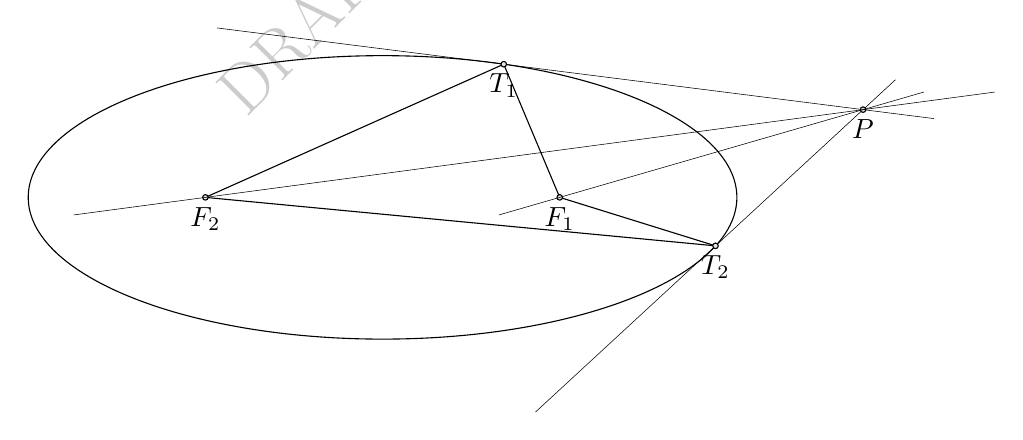
\begin{tikzpicture}[scale=0.9]
  \draw (0,0) ellipse (5 and 2) ;
  \tkzDefPoint(2.5,0){F1} \tkzDefPoint(-2.5,0){F2}
  \node[inner sep=0pt] (a) at ($(0,0)+(70:5 and 2)$) {} ;
  \draw (a) -- (-2.5,0) ; \draw (a) -- (2.5,0) ;
  \node[inner sep=0pt] (b) at ($(0,0)+(-20:5 and 2)$) {} ;
  \draw (b) -- (-2.5,0) ; \draw (b) -- (2.5,0) ;
  \tkzLabelPoint(F1){$F_1$}
  \tkzLabelPoint(F2){$F_2$}
  \tkzLabelPoint(a){$T_1$}
  \tkzLabelPoint(b){$T_2$}

  \tkzDefEquilateral(a,F1) \tkzGetPoint{C}
  \tkzDrawLine[add=2 and 2](a,C)

  \tkzDefEquilateral(b,F1) \tkzGetPoint{D}
  \tkzDrawLine[add=1.5 and .5](b,D)

  % Cette construction cache le fait que l'angle entre le fait que
  % l'angle PaF1 mesure 60° ?

  \tkzInterLL(a,C)(b,D) \tkzGetPoint{P}
  \tkzDrawPoints(a,b,F1,F2,P)
  \tkzLabelPoints(P)

  \tkzDrawLine(P,F1) \tkzDrawLine(P,F2)

\end{tikzpicture}

Soit une ellipse (respectivement une hyperbole) de foyers $F$ et $F'$.

\begin{proposition}
  En tout point $M$ d'une ellipse (respectivement d'une hyperbole), la
  tangente est la bissectrice extérieure (respectivement intérieure) de
  l'angle $\widehat{FMF'}$.
\end{proposition}

\begin{proof}[dans le cas de l'ellipse]
  $MF+MF'=2a$

  $\lVert MF\rVert + \lvert F'F +FM\rVert = 2a$

  On suppose qu'on dispose d'un paramétrage de classe $\mathcal{C}^1$ de
  l'ellipse. En dérivant, on a:

  $\frac{FM\cdot\frac{\mathrm{d}M}{\mathrm{d}t}}{\lVert FM\rVert} +
  \frac{F'M\cdot\frac{\mathrm{d}M}{\mathrm{d}t}}{\lVert F'M\rVert} = 0$

  $\left(\frac1{\lVert FM\rVert}FM + \frac1{\lVert F'M\rVert}F'M\right)
  \cdot \frac{\mathrm{d}M}{\mathrm{d}t}$

  On peut poser $n=\frac1{\lVert FM\rVert}FM$ et de même pour $n'$ qui
  sont ainsi deux vecteurs unitaires. Ils définissent ainsi l'angle
  $\widehat{F'MF}$ et $n+n'$ est la bissectrice intérieure de cet angle.

  On en tire que la tangente en $M$, c'est à dire
  $\frac{\mathrm{d}M}{\mathrm{d}t}$ est précisément orhtogonale à la
  bissectrice intérieure, c'est donc la bissectrice extérieure.
\end{proof}

\begin{proof}[dans le cas de l'hyperbole]
  On reprends les calculs précédents dans le cas $MF-MF'=2a$ ou
  $MF'-MF=2a$, ce qui nous conduit, avec les notations de la proof
  précédente, à $n-n'$ orthogonale à la tangente.
\end{proof}
\end{document}
